\begin{figure}
\caption{Smoothed Estimates of Structural Shocks}\label{fg:shocks}
\vspace*{1pc}\hspace*{-0.2in}
\begin{tabular}{ccc}
\multicolumn{3}{c}{Case 1: Rational Expectations} \\ 
Natural Rate & Cost-Push & Monetary Policy \\
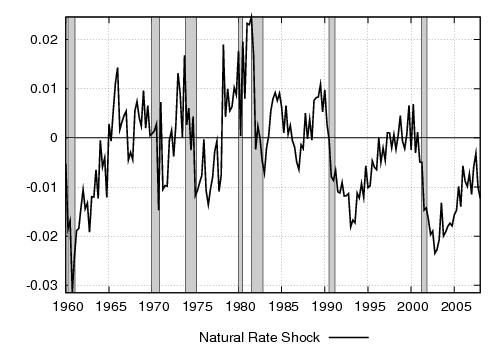
\includegraphics[scale=0.3]{results_re/natrateshock.png} & 
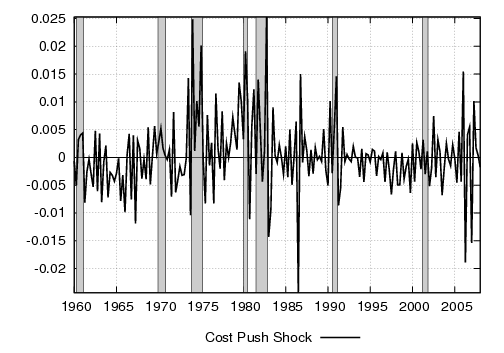
\includegraphics[scale=0.3]{results_re/costpushshock.png} & 
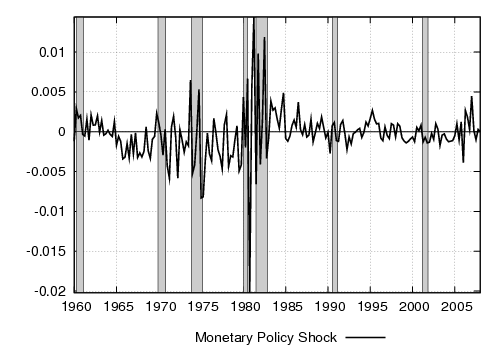
\includegraphics[scale=0.3]{results_re/mpshock.png} \\ \\ 
 
\multicolumn{3}{c}{Case 2: Learning with RE Initial Conditions} \\ 
Natural Rate (0.9752) & Cost-Push (0.9434) & Monetary Policy (0.9629) \\
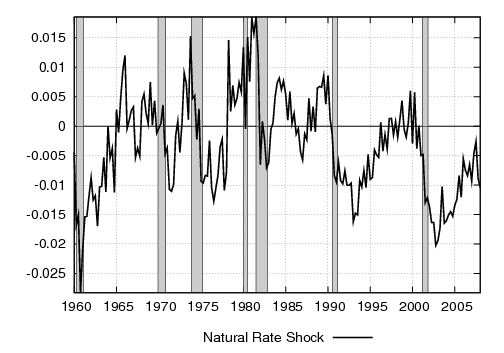
\includegraphics[scale=0.3]{results_reallinit/natrateshock.png} & 
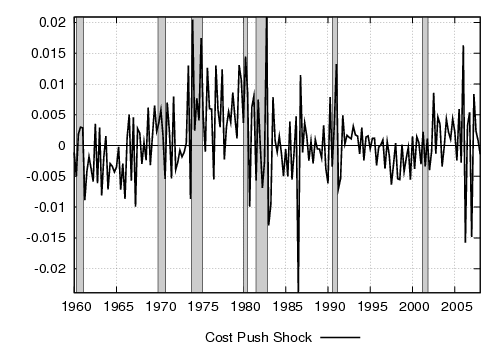
\includegraphics[scale=0.3]{results_reallinit/costpushshock.png} & 
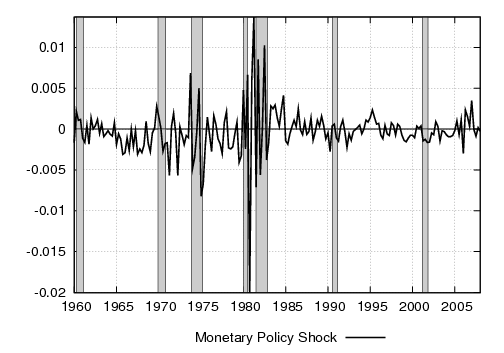
\includegraphics[scale=0.3]{results_reallinit/mpshock.png} \\ \\ 
 
\multicolumn{3}{c}{Case 3: Learning with Unobservable Shocks and RE Initial Conditions} \\ 
Natural Rate (0.8366) & Cost-Push (0.9343) & Monetary Policy (0.8062) \\
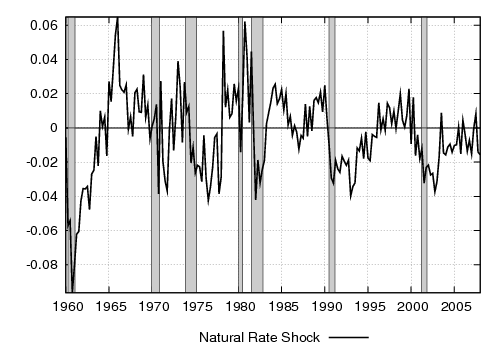
\includegraphics[scale=0.3]{results_reinit/natrateshock.png} & 
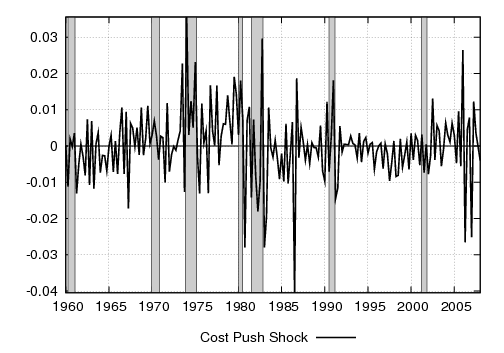
\includegraphics[scale=0.3]{results_reinit/costpushshock.png} & 
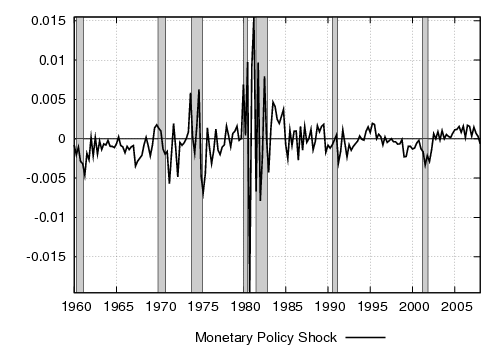
\includegraphics[scale=0.3]{results_reinit/mpshock.png} \\ \\ 
 
\multicolumn{3}{c}{Case 4: Learning with Unobservable Shocks and Pre-Sample Initial Conditions} \\ 
Natural Rate (0.6217) & Cost-Push (0.9071) & Monetary Policy (0.8383) \\
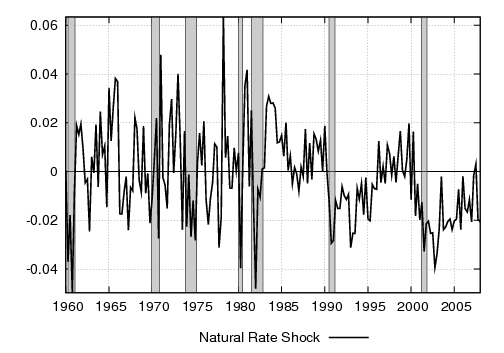
\includegraphics[scale=0.3]{results_wlsinit/natrateshock.png} & 
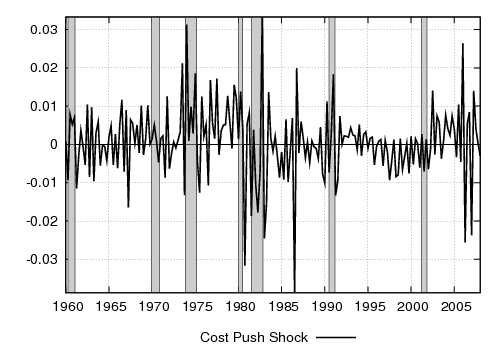
\includegraphics[scale=0.3]{results_wlsinit/costpushshock.png} & 
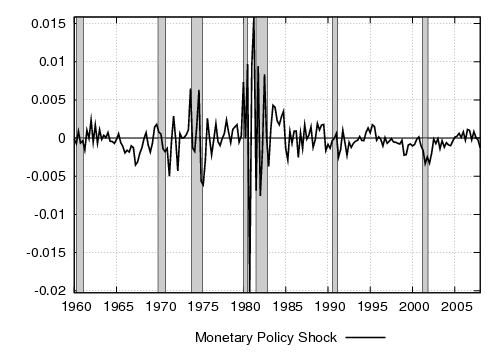
\includegraphics[scale=0.3]{results_wlsinit/mpshock.png} \\ \\ 
 
\end{tabular}
\end{figure}
